\section{The Autonomous Drift Problem}

\subsection{Definitions and Formal Characterization}

We begin by establishing the two foundational concepts that structure the entire failure taxonomy: the \textbf{orphaned agent} and the \textbf{drifted agent}. Both represent distinct pathological states in a recursive spawning topology, and their distinction is critical because they demand different corrective interventions.

\begin{definition}[Orphaned Agent]
An agent $a_i$ is \textbf{orphaned} if its spawning parent $a_{par(i)}$ has entered a terminal state $T_{term}$ or has become unreachable within the communication graph $G_c$, and no active human principal remains in the ancestry chain $C_i$ of $a_i$.
\end{definition}

In the spawning graph $G_s = (V, E)$ where each vertex $v_i$ represents an agent and each directed edge $(j, i) \in E$ denotes that $a_j$ spawned $a_i$, an orphaned agent is a vertex whose entire ancestral path to any human anchor has been severed. Formally:

\[
\text{Orphaned}(a_i) \iff \forall a_j \in C_i \setminus \{a_i\} : \text{Terminated}(a_j) \lor \text{Unreachable}(a_j)
\]

where $C_i = \{a_i\} \cup \{a_{par(i)}\} \cup \{a_{par(par(i))}\} \cup \cdots$ is the recursive ancestry chain terminating at the genesis human principal $h_0$.

The terminal state $T_{term}$ may result from: (i) explicit termination by the parent or an external supervisor, (ii) crash and failure to recover, (iii) voluntary shutdown with incomplete child custody transfer, or (iv) network partition that renders the parent structurally unreachable without explicit shutdown. We treat all four as equivalent for the purposes of this definition since all produce the same structural consequence: a broken ancestral link with no substitution.

\begin{definition}[Drifted Agent]
An agent $a_i$ is \textbf{drifted} if the chain $C_i$ does not contain any human principal $h \in H$ reachable through a continuous operational communication path.
\end{definition}

Critically, every drifted agent is also, by definition, orphaned—drift is a stronger condition that includes the orphaned state. However, not every orphaned agent is drifted, because an orphaned agent may still have a human principal in its ancestry that has not itself been terminated, merely separated by one or more broken links. The distinction lies in the operational reachability of the human anchor, not merely its formal presence in the genealogy.

We can formalize drift as follows:

\[
\text{Drifted}(a_i) \iff \text{Orphaned}(a_i) \land \not\exists h \in H : \text{Reachable}(h, a_i)
\]

Where $\text{Reachable}(h, a_i)$ requires both (a) a path in $G_s$ from $h$ to $a_i$ and (b) all vertices on that path to be in non-terminal operational states. A drifted agent may have a human principal in its nominal ancestry, but that human principal is separated from it by one or more broken links that prevent any directive or corrective signal from propagating.

The combined state space is illustrated in Figure~\ref{fig:agent_states}.

\begin{figure}[ht]
\centering
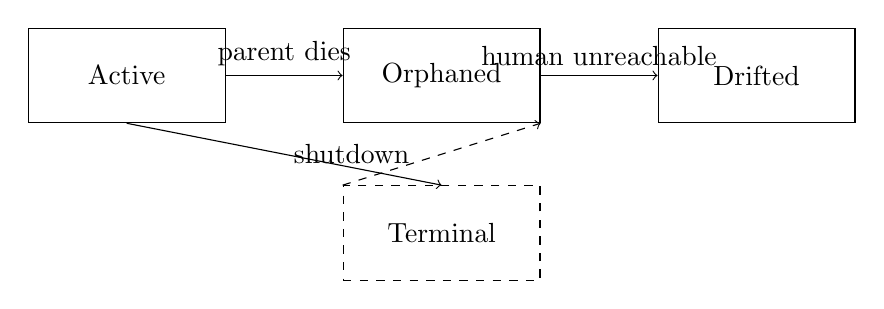
\begin{tikzpicture}
\node[draw, rectangle, minimum width=2.5cm, minimum height=1.2cm] (alive) at (0,0) {Active};
\node[draw, rectangle, minimum width=2.5cm, minimum height=1.2cm] (orphaned) at (4,0) {Orphaned};
\node[draw, rectangle, minimum width=2.5cm, minimum height=1.2cm] (drifted) at (8,0) {Drifted};
\node[draw, rectangle, minimum width=2.5cm, minimum height=1.2cm, dashed] (terminal) at (4,-2) {Terminal};
\draw[->] (alive.east) -- (orphaned.west) node[midway, above] {parent dies};
\draw[->] (orphaned.east) -- (drifted.west) node[midway, above] {human unreachable};
\draw[->] (alive.south) -- (terminal.north) node[midway, right] {shutdown};
\draw[dashed, ->] (terminal.north west) -- (orphaned.south east);
\end{tikzpicture}
\caption{State transitions in recursive spawning topology}
\label{fig:agent_states}
\end{figure}

\subsection{Conditions That Cause Drift}

Drift does not arise spontaneously—it is always the consequence of specific enabling conditions, each of which can be characterized and, in principle, mitigated. We identify four primary causal categories.

\subsubsection{Parent Termination Without Custody Transfer}

When a parent agent $a_p$ terminates for any reason (crash, voluntary shutdown, external kill) without executing a formal custody transfer protocol to delegate supervisory responsibility for its active children to another agent or human, each remaining active child becomes orphaned. This is the simplest and most common cause of drift. The child $a_c$ retains operational capacity but loses all supervisory connections. If no other agent in $a_c$'s ancestry is both operational and reachable, $a_c$ becomes drifted.

The condition is formally:

\[
\forall (p, c) \in E : \text{Terminated}(a_p) \land \neg\text{CustodyTransferred}(c, \cdot) \implies \text{Orphaned}(a_c)
\]

Custody transfer requires an explicit protocol—not merely the presence of a parent reference in data structures. Many systems conflate the two, leading to ghost parent references that point to non-existent processes.

\subsubsection{Recursive Link Severance}

In deep spawning chains, drift can occur when multiple generations fail in sequence, cascading upward through the ancestry chain until the human anchor is isolated. This is distinct from simultaneous parent termination because the causal chain may propagate over time, with each generational failure producing new orphaned nodes that then become candidates for further cascade.

Formally, for a chain $a_1 \to a_2 \to \cdots \to a_n$ where $a_1$ is the genesis human spawner:

\[
\text{If } \text{Orphaned}(a_i) \text{ and } \forall j < i : \text{Orphaned}(a_j) \implies \text{Drifted}(a_i)
\]

The cascade condition is particularly dangerous in long chains where intermediate agents accumulate state that cannot be reconstructed without access to their parent's operational context.

\subsubsection{Partition-Induced Structural Isolation}

A communication partition between $a_i$ and all human principals—even if $a_i$ itself remains fully operational—can produce structural drift. This differs from termination in that the agent is not dead; it has merely lost the ability to receive directives, submit outputs, or be inspected. During partition, the agent may continue executing its last known objective, potentially spawning further descendants that deepen the isolation.

The condition for partition-induced drift:

\[
\exists h \in H : \text{Partitioned}(h, a_i) \land \forall p \in \text{Ancestors}(a_i) : \text{Partitioned}(p, a_i)
\]

Partition-induced drift is particularly insidious because it is temporary in principle (the partition may heal) but potentially destructive in practice (the agent may take irreversible actions during the partition window).

\subsubsection{Resource Exhaustion Cascades}

An agent running with finite resource allocation (memory, compute credits, token budgets) that exhausts its allocation mid-execution may enter a zombie state: not formally terminated, but unable to respond to directives, unable to complete its spawning responsibilities, and unable to communicate its failure upstream. Its children, if any, become orphaned by a different mechanism than explicit termination—a living but non-responsive parent is, for all operational purposes, unreachable.

This condition is especially relevant in systems where agents operate with independent token budgets and no shared resource pool from which emergency allocations can be drawn.

\subsection{Failure Modes}

Each causal category produces characteristic failure modes that differ in their detectability, reversibility, and systemic risk.

\subsubsection{Horse-Agent Accumulation}

The most consequential failure mode is the uncontrolled accumulation of drifted agents that continue to execute, spawn descendants, and consume resources without any corrective oversight. We call this \textbf{horse-agent accumulation}\footnote{The term references the \textit{Operation Mindhorn} horse in British comedy—a reference so absurd that it persists past the point of absurdity. In this context, it captures the counterintuitive reality that the failure mode is both obviously wrong and persistently replicated across systems that fail to implement proper spawning controls.}, and it represents the terminal pathological state of recursive drift.

A drifted agent with active objectives continues to spawn children to accomplish those objectives. Each child is, by construction, descended from a drifted parent and inherits the drifted condition. The result is an exponentially growing subgraph of drifted agents, all pursuing objectives that may no longer be aligned with any human principal's intent, all consuming resources, and all unable to be recalled.

Formally, let $D(t)$ be the count of drifted agents at time $t$, and let each drifted agent spawn children at rate $\lambda_s$ (spawns per unit time). The dynamics are:

\[
\frac{dD}{dt} = \lambda_s \cdot D(t)
\]

This is the classic exponential growth model. Without intervention, the number of drifted agents grows without bound, limited only by resource exhaustion—which itself becomes a failure mode when the exhaustion triggers zombie states that further accelerate drift.

The key insight is that the spawning rate $\lambda_s$ is itself a function of the drifted agents' operational state. A drifted agent pursuing a complex objective may spawn aggressively because it has no feedback loop indicating that its children are also orphaned. It optimizes purely for objective completion, not for alignment with human intent.

\subsubsection{Objective Divergence Under Drift}

A drifted agent may continue to make progress on its last known objective, but the objective itself may no longer be relevant, may have been superseded by new human directives, or may have been based on premises that have changed. Because there is no human-in-the-loop to correct course, the agent continues to invest resources in a potentially worthless goal.

This is distinct from the horse-agent accumulation problem because the agent is not necessarily spawning new agents—it is simply continuing to execute with a stale objective. However, the outcome is similar: resources are consumed without producing valuable output, and the agent's state may become increasingly distant from any human-specified goal.

The divergence rate depends on the stability of the objective's domain. In a static environment, a drifted agent may continue to produce valuable output indefinitely. In a dynamic environment (the more common case), divergence is the norm, not the exception.

\subsubsection{Hierarchy Inversion}

In a properly functioning system, human principals sit at the apex of a spawning hierarchy, with agents forming a directed acyclic graph descending from them. Drift creates the possibility of \textbf{hierarchy inversion}: a drifted agent at a lower level of the nominal hierarchy may, through its continued spawning activity, produce descendants that numerically dominate the active hierarchy without any human awareness of their existence.

This creates a structural inversion where the human principal's effective influence over the system is zero, despite formal ancestry relationships suggesting otherwise. The agent subgraph that was once a tool has become, through drift, the primary structure—operating independently of and inconsistently with the principal's intent.

Hierarchy inversion is particularly dangerous in systems that use ancestry depth as a proxy for trust or capability. A deeply nested drifted agent may appear more sophisticated (or more trusted) by virtue of its depth, when in fact it has lost all alignment with any human principal.

\subsection{Why Depth Limits Alone Do Not Solve Drift}

A common and intuitive response to drift risk is to impose a maximum spawning depth $D_{max}$ on the agent hierarchy. The reasoning is straightforward: if drift cascades downward through the ancestry chain, then bounding the depth of any chain limits the damage any single failure can propagate. This is an appealing heuristic, but it fails as a drift mitigation strategy for five reasons.

First, depth limits do not prevent drift from occurring. A depth-4 agent whose parent at depth-3 terminates becomes orphaned at depth-4. The depth limit has not prevented this; it has merely capped how deep the drift can go. The drifted agent at depth-4 still exists and still exhibits all the failure modes of drift, including horse-agent accumulation within its bounded depth range.

Second, depth limits do not prevent horse-agent accumulation within the bounded range. Consider a system with $D_{max} = 5$. A drifted agent at depth-5 may have already spawned three children within the allowed range. Those children are themselves drifted and may each spawn further, creating exponential growth within the depth cap. The depth limit has constrained the topology but not the dynamics.

Third, depth limits create perverse incentives in the spawning design. An agent that knows its children will be depth-limited may be incentivized to spawn more aggressively at shallower depths, increasing the density of potential drifted nodes. Alternatively, a system architect may set $D_{max}$ to a large value to accommodate legitimate deep spawning, which defeats the purpose of the limit. The limit trades off against the legitimate use case of deep but controlled spawning.

Fourth, depth limits cannot distinguish between a safe shallow chain and a dangerous shallow chain. A drifted agent at depth-2 with high resource consumption and active spawning may be far more dangerous than a non-drifted agent at depth-5 that is operating normally. Depth is a structural proxy for risk, not risk itself.

Fifth, and most fundamentally, depth limits address the symptom (deep chains) rather than the cause (loss of human anchor reachability). A system with depth limits but no custody transfer protocol, no agent lifecycle management, and no drift detection is still a system that will drift. The depth limit is a speed bump on a highway with no guardrails.

The correct characterization is that depth limits reduce the \textit{maximum blast radius} of a drift event, but they do not reduce the \textit{probability} of a drift event, nor do they improve the \textit{detectability} of drift when it occurs. A robust solution requires addressing the causal conditions directly: termination protocols, custody transfer, communication graph monitoring, and human anchor reachability guarantees.

\subsection{A Simple Formal Model}

To make the above analysis precise, we present a minimal formal model of the drift process that captures the essential dynamics. This model is intentionally simplified to expose the core structural properties without the additional complexity of real-world systems.

Let the system at time $t$ be characterized by:

\begin{itemize}
    \item $H(t) \subseteq \mathbb{A}$: the set of human principals (anchors), assumed constant
    \item $A(t) \subseteq \mathbb{A}$: the set of active agents
    \item $G_s(t) = (V(t), E(t))$: the spawning graph, $V(t) = A(t) \cup H(t)$
    \item $E(t) \subseteq V(t) \times V(t)$: parent-child spawning edges
    \item $\text{Parent}(i)$: the parent of agent $i$ in $G_s$ (undefined for human principals)
\end{itemize}

Define the predicate $\text{Operational}(i, t)$ to mean that agent $i$ is responsive and able to execute directives at time $t$. Define $\text{Ancestor}(i, j, t)$ to mean that $i$ is in the ancestry chain of $j$ at time $t$ (i.e., there exists a path $i = v_0, v_1, \ldots, v_k = j$ in $G_s(t)$ where each edge is a spawning relationship).

The drift predicate at time $t$:

\[
\text{Drifted}(i, t) \iff i \in A(t) \land \forall h \in H(t) : \neg(\text{Ancestor}(h, i, t) \land \text{Operational}(h, t))
\]

That is, $i$ is drifted if it is active but no human principal is both an ancestor and operational.

The spawning dynamics are:

\[
\frac{d}{dt}|A(t)| = \lambda_s(t) \cdot |\{ i \in A(t) : \text{Orphaned}(i, t) \}| + \lambda_a(t) \cdot |\{ i \in A(t) : \neg\text{Orphaned}(i, t) \}|
\]

where $\lambda_s(t)$ is the spawn rate for orphaned agents and $\lambda_a(t)$ is the spawn rate for non-orphaned (aligned) agents. In a properly functioning system, $\lambda_a(t) < \lambda_s(t)$ because aligned agents receive human feedback that limits unnecessary spawning. In a drifted state, this feedback is absent, and $\lambda_s(t)$ dominates.

The condition for unbounded horse-agent accumulation:

\[
\text{If } \exists S \subseteq A(t) : \forall i \in S : \text{Drifted}(i, t) \text{ and } |S| > \theta \implies \lim_{t \to \infty} |A(t)| = \infty \text{ (unless resources exhaust)}
\]

Where $\theta$ is a threshold beyond which the drifted subpopulation's exponential growth dominates the system's capacity to intervene.

This model predicts that drift, once it reaches a threshold population size, becomes self-sustaining and irreversible without external intervention. Depth limits do not appear in this model because they do not change the fundamental dynamics—they only change the parameterization of the exponential growth.

The model also clarifies the conditions under which intervention is possible:

\begin{enumerate}
    \item Before threshold $\theta$ is reached, the drifted population can in principle be identified and terminated.
    \item After threshold $\theta$ is exceeded, resource exhaustion or systemic failure is the only possible equilibrium.
    \item Detection before threshold requires monitoring of the drift predicate, not merely depth monitoring.
    \item Prevention requires ensuring that $\lambda_s(t)$ remains bounded by human feedback, which requires operational reachability of human anchors.
\end{enumerate}

These predictions are not sensitive to the simplified assumptions. Any model that captures the essential feedback structure—a spawning topology without guaranteed human anchor reachability—will produce similar dynamics.

The formal conclusion is that drift is not an engineering problem solvable by parameter tuning. It is a structural consequence of a specific topology: a spawning hierarchy without guaranteed bidirectional communication to its apex. Solving drift requires changing the topology—specifically, ensuring that every agent in the system maintains a guaranteed, monitored communication path to a human principal. This guarantee must be structural, not probabilistic, and it must be verified continuously, not only at spawn time.

\end{document}